\section{Methodology}

\begin{figure}[h]
	\center
	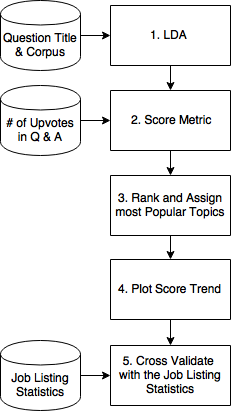
\includegraphics[width=5cm]{flowChart}
    \caption{General flowchart of the proposed algorithm}
    \label{fig:flowChart}
\end{figure}


\subsection{Data collection}
To analyze the score trend of the selected topics. We download the Q\&A entries from Stack Overflow and US technology job listing dataset from Kaggle.com. The file was separated by year, starting from 2008 to 2014. The title and corpus of the question entries were used for topic categorization with LDA. The upvotes of questions and upvotes of answers were extracted to calculate the score.

\subsection{Algorithm design}
The flowchart of the algorithm is shown in figure \ref{fig:flowChart}. The first step of the approach is to apply LDA algorithm to the titles and corpus of question entries. The granularity constant K will be tuned to lower the variance of the topic numbers in each category.
With the generated unnamed categories, the second step incorporated the votes of the questions and answers to calculate scores for each category.
In the third step, the categories with the top scores of all times from 2008 to 2014 were named according to the LDA most frequent keywords. Only the top scored topics were plotted in the trend comparison.
The score trend for the top ranked topics were plotted from 2008 to 2014. In our hypotheses, the score of the topics should match to the future popularities of the corresponding jobs.


%\subsection{Language and tool used}
We will mainly use python in this course project. Multiple open source packages would be used, including but not limited to pandas, NLTK, stop\_words, and genism. We will use the online tutorial "Latent Dirichlet Allocation (LDA) with Python" \cite{T1_Paper} as a reference to apply the LDA algorithm. 



%\subsubsection{a prototype (optional if time permit)}

\subsection{Scoring metric}

The scoring of the topics was calculated based on the supply and demand of the skills. High score indicates that the topic is popular with limited skill support. The score metric formula was designed as:

\begin{equation} \label{eq:1}
	Score = \frac{Demand - Supply}{n}
\end{equation}

$Demand$ is the number of upvotes in questions, $Supply$ is the number of upvotes in Answers, and $n$ is the number of entries, which normalizes the score for that specific topic. 

The voting system in Stack Overflow subtracted the downvotes from the upvotes. The cancellation effect automatically takes the downvotes into account. The formula is based on the assumption that the number of question upvotes could fully represent the demand while the number of answer upvotes represent the supply of talent in that specific topic.


\subsection{Testing against hypothesis}
To test against the hypothesis, we will check if the rank of the topic will predict the future popularity of  job fields by comparing the shape of the score curves with the job listing trends. Currently we have not decided on the source of the job listing statistics because the job titles have to fit in the categories summarized by the keywords generated from the LDA analysis. We will start searching the data when we obtain the results of the most popular topics from the LDA.


%\subsection{how to proof correctness (required by dissertation only)}